\documentclass[11pt]{article}

\usepackage[T1]{fontenc}
\usepackage[utf8]{inputenc}
\usepackage{lmodern}
\usepackage{geometry}
\usepackage{graphicx}
\usepackage{amsmath}

\geometry{margin=1in}
\pagenumbering{gobble}

\begin{document}

\begin{center}
    {\Large \textbf{Residual Structure in Rydberg CZ Gate Benchmarking}} \\
    \vspace{6pt}
    \normalsize Dan Hawkley
\end{center}

\vspace{10pt}

\begin{center}
    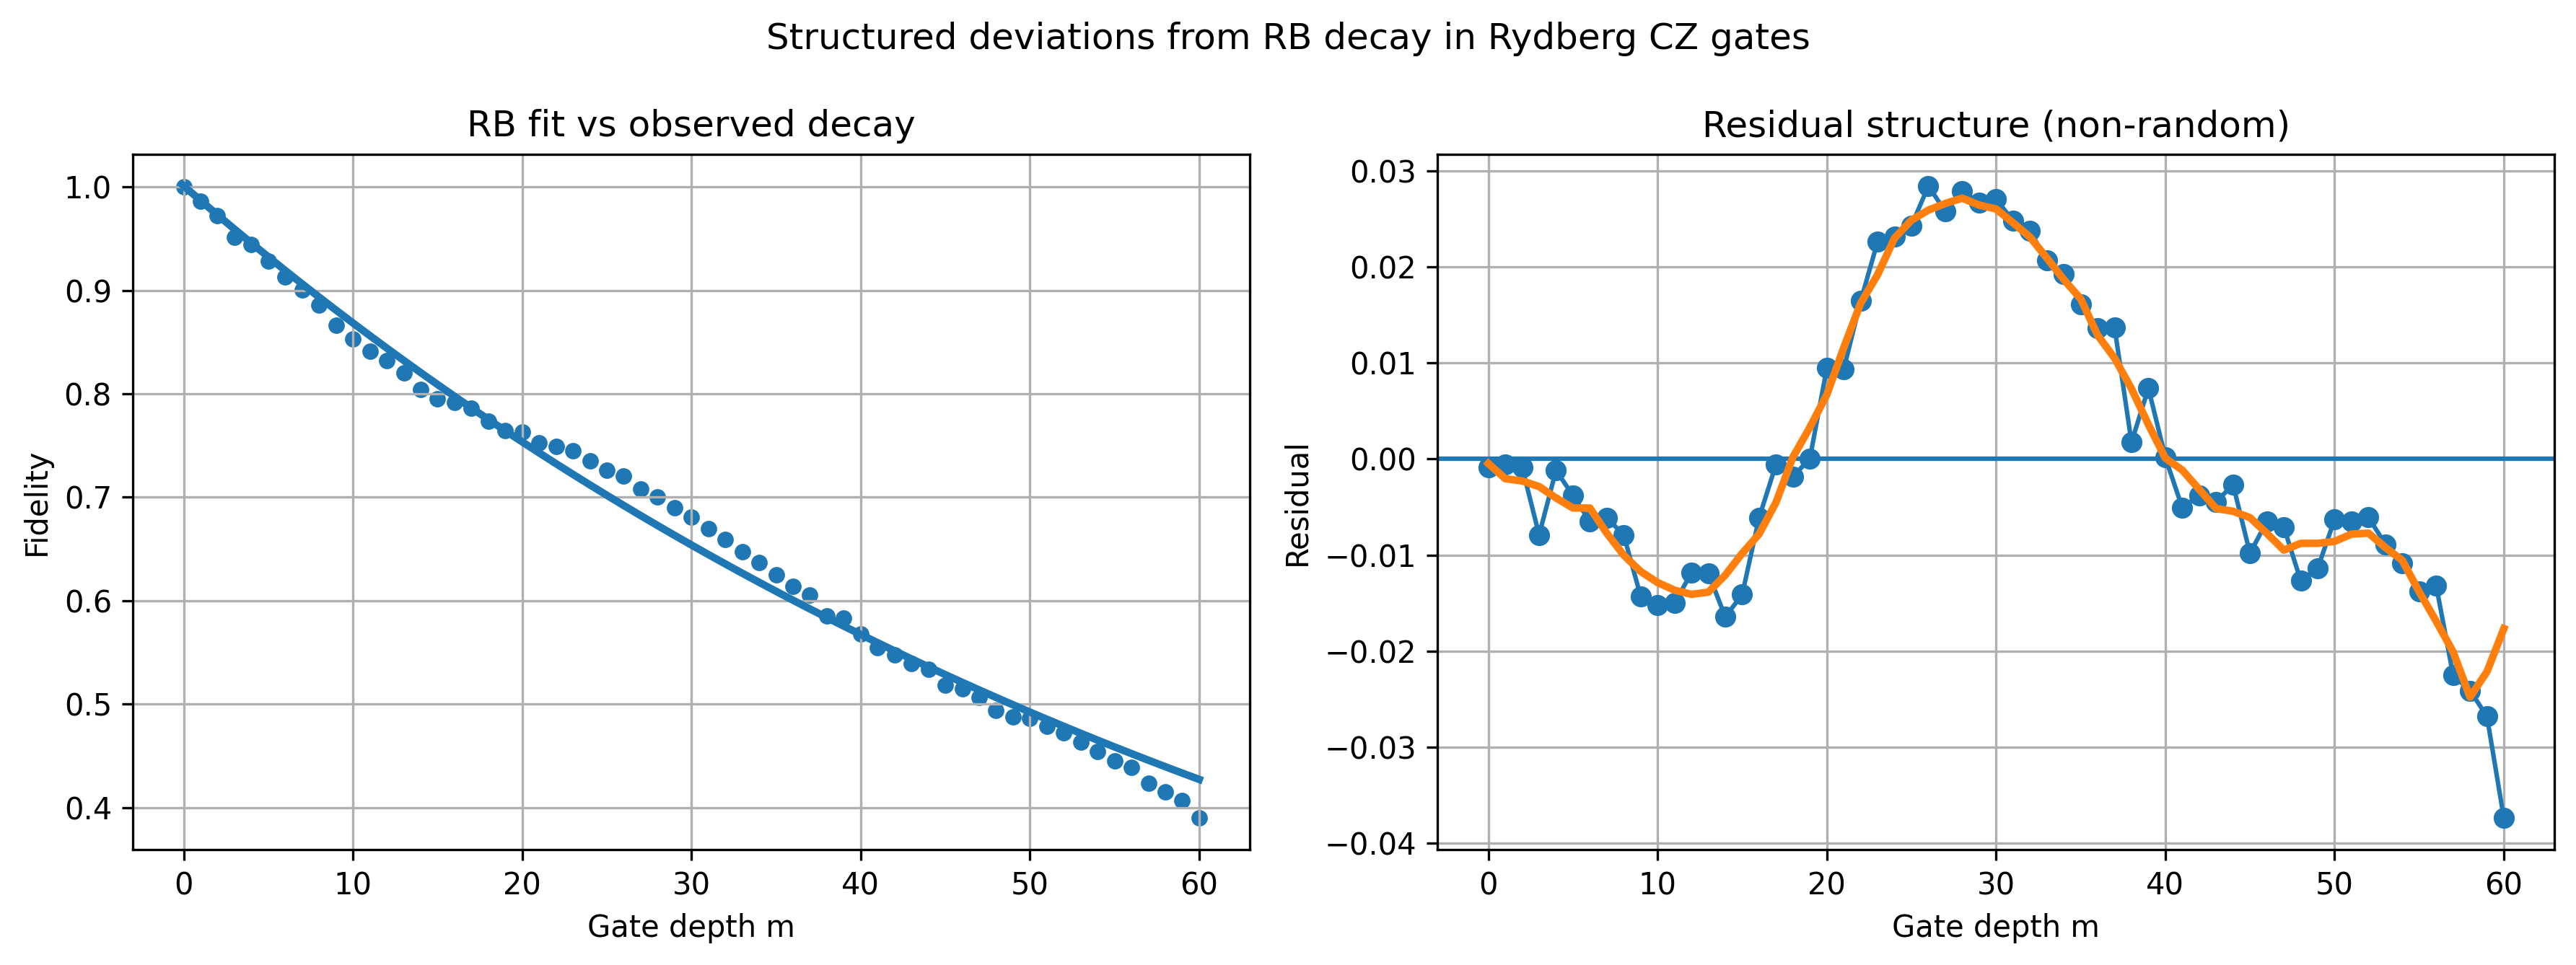
\includegraphics[width=\textwidth]{residual_structure.png}
    
    \vspace{4pt}
    \small
    Structured deviations from RB decay in Rydberg CZ gates:
    left — RB fit captures overall decay;
    right — residuals show clear non-random structure.
    \normalsize
\end{center}

\vspace{10pt}

\noindent
Randomized benchmarking (RB) is commonly used to characterize quantum gate performance
by fitting fidelity decay to an exponential form,
\[
F(m) = A p^m + B.
\]
This compresses behavior into a single decay parameter $p$, which is often interpreted
as an average error rate.

\vspace{6pt}

\noindent
In this Rydberg CZ gate model, the RB fit (left panel) captures the overall decay trend,
but the residuals (right panel) exhibit clear structure rather than random noise.
This indicates that the underlying dynamics are not fully described by a simple
exponential decay model.

\vspace{6pt}

\noindent
The residual structure suggests the presence of coherent or non-Markovian effects,
which can arise from control imperfections, dephasing, or interaction-driven dynamics.
To organize these effects, we introduce an effective noise coordinate,
\[
\gamma_{\mathrm{eff}} = \gamma + \lambda \gamma_{\phi}.
\]
This combines incoherent and dephasing contributions.

\vspace{6pt}

\noindent
This example illustrates a key point for quantum characterization:
while RB provides a useful summary of gate performance, structured residuals
contain additional information about the physical noise processes.

\vspace{6pt}

\noindent
\textbf{Conclusion:} residuals are not just fitting error—they are signal.

\end{document}